\documentclass[conference]{IEEEtran}
\hbadness=10000
\vbadness=10000
\usepackage{cite}
\usepackage{amsmath,amssymb,amsfonts}
\usepackage{graphicx}
\usepackage{textcomp}
\usepackage{xcolor}
\usepackage{booktabs}
\usepackage{multirow}
\usepackage{url}
\usepackage{algorithm}
\usepackage{algpseudocode}
\usepackage{hyperref}
% \documentclass{standalone}
\usepackage{tikz}
\usetikzlibrary{shapes,arrows,positioning,calc,fit,backgrounds}
% Keep the paper buildable when optional experiment exports are unavailable.
\newcommand{\experimentfigure}[2][]{%
    \IfFileExists{#2}{\includegraphics[#1]{#2}}{%
        \fbox{\parbox[c][3.0cm][c]{0.94\linewidth}{\centering
        Experiment figure unavailable:\\[0.3em]\texttt{\detokenize{#2}}}}%
    }%
}

\def\BibTeX{{\rm B\kern-.05em{\sc i\kern-.025em b}\kern-.08em
    T\kern-.1667em\lower.7ex\hbox{E}\kern-.125emX}}


\begin{document}

\title{A WGAN-GP and Denoising Diffusion Hybrid for Denoising and Super-Resolution on CelebA}

\author{
    \IEEEauthorblockN{
        Ahmed Faizul Haque Dhrubo\textsuperscript{*}, 
        S.M. Riaz Rahman Antu, 
        Saif Ahmed, 
        Ashadulla Hil Galib, \\ 
        Mohammad Abdul Qayum, 
        Mohsin Sajjad, 
        Mohammad Ashrafuzzaman Khan,
        and Souvik Pramanik
    }
    \IEEEauthorblockA{
        \textit{Department of Electrical and Computer Engineering}\\
        \textit{North South University},Dhaka, Bangladesh \\
        {\{ahmed.dhrubo, riaz.antu, saif.ahmed03, ashadulla.galib}, \\{mohammad.qayum, mohsin.sajjad, mohammad.khan02, souvik.pramanik\}}@northsouth.edu
    }
}


\maketitle

\begin{abstract}
Generative adversarial networks (GANs) can provide efficient image generation, while diffusion models offer high-quality image restoration but require iterative sampling. This paper presents a hybrid GAN-guided diffusion framework that uses a pretrained Wasserstein GAN with gradient penalty (WGAN-GP) as a feature prior for conditional diffusion-based image restoration. Intermediate features from the frozen WGAN-GP generator are incorporated into a diffusion U-Net through cross-attention and remain fixed during the DDIM sampling process. The framework is evaluated on two restoration tasks, Gaussian denoising and $2\times$\textit{super-resolution}, using CelebA face images. During development, several sources of instability were identified and addressed, including adversarial learning-rate imbalance, inappropriate diffusion initialization, excessive corruption, and insufficient parameter averaging. The resulting framework consistently improves the quality of both degraded and low-resolution images. In particular, it improves denoising performance by 4.40 dB in PSNR and super-resolution performance by 3.70 dB over their respective input baselines. These results demonstrate the potential of a frozen GAN feature prior to guide diffusion models toward stable and effective image restoration.
\end{abstract}

\begin{IEEEkeywords}
generative adversarial networks, diffusion models, image restoration, image denoising, super-resolution, WGAN-GP, cross-attention
\end{IEEEkeywords}

\section{Introduction}
Deep generative models have emerged as essential tools for image synthesis and recovery, and two types of such models, namely generative adversarial networks (GANs) and diffusion models, complement each other. In particular, GANs \cite{goodfellow2014gan} generate images using only one forward pass and thus provide efficient inference. Objective functions based on Wasserstein distance with gradient penalty, for example WGAN-GP \cite{gulrajani2017wgangp}, also provide additional benefits in terms of stable training. On the other hand, GANs may still exhibit mode collapse, oscillations during training, and instability due to the interplay between the learning dynamics of the generator and the discriminator. Diffusion probabilistic models (DDPMs) \cite{ho2020ddpm, sohl2015deep} serve as another method of image generation by training a model to reverse the noising process in a series of denoising steps. While diffusion models show high accuracy and high variety \cite{dhariwal2021diffusion}, their iterative nature of image generation requires much higher computational efforts than the one-time generation performed by GANs. Diffusion models may experience instability with poor initialization and restricted settings, whereas GANs are highly capable of modeling structural and semantic manifolds. Integrating the two approaches capitalizes on the strengths of both by allowing a pretrained GAN to serve as a supplementary feature-level prior for the diffusion model's optimization iterations without compromising its restoration procedure. With this in mind, this paper suggests a GAN-aided diffusion model for Gaussian denoising and $2\times$ super-resolution using a WGAN-GP generator that has been pretrained on CelebA faces and is later frozen before being plugged into a conditional diffusion U-Net via cross-attention to provide facial structure guidance while maintaining the denoising ability. This final architecture was empirically developed based on multiple iterations—first, deciding which architecture of GAN is to be used out of DCGAN, WGAN-GP, and StyleGAN-lite (which resulted in choosing WGAN-GP for stability and quality reasons) and then resolving issues arising in training and inference due to generator-critic learning rates, DDIM initialization, corruption strength, and exponential moving average smoothing.
\begin{figure}
    \centering
    \includegraphics[width=1.0\linewidth]{visual_abs.pdf}
    \label{fig:visabs}
\end{figure}


The main goal of this work is to examine whether a pre-trained WGAN-GP provides an adequate feature-level prior for conditional diffusion-based image restoration through the design of a hybrid approach in which intermediate spatial features of the frozen GAN generator steer the diffusion U-Net via cross-attention. The second goal is to apply this architecture to the tasks of Gaussian image denoising and $2\times$ super-resolution as two distinct low-level vision problems. Moreover, it is necessary to uncover and mitigate pipeline instabilities associated with the proper tuning of the adversarial learning rate ratio, diffusion initialization, corruption normalization, and exponential moving averages.


This paper proposes a novel GAN-prior guided conditional diffusion network, in which a frozen WGAN-GP generator generates the intermediate spatial features before the diffusion U-Net through cross-attention, calculated once for each sampling chain and fixed during the DDIM sampling process. For the stability of the model, this paper gives a diagnosis-driven solution to the following problems: the imbalance between the learning rate of generator and critic, DDIM initialization problem, excessive corruption intensity, and lack of EMA smoothing. We evaluate the effectiveness of our learned GAN-prior for image restoration on Gaussian denoising and $2\times$ super-resolution tasks on the CelebA dataset.


\section{Related Work}

Modern techniques of image restoration have become more inclined towards the use of GANs together with diffusion models. The use of DCGAN \cite{radford2015dcgan} and StyleGAN \cite{karras2019stylegan} have led to the development of strong convolutional and style-based generator functions that provide realistic samples. At the same time, WGAN-GP \cite{gulrajani2017wgangp}, which is based on Wasserstein critic and gradient-norm regularizer, almost eliminates mode collapsing. On the contrary, diffusion models, which were first proposed by Sohl-Dickstein et al. \cite{sohl2015deep} and later described theoretically by Ho et al. \cite{ho2020ddpm} as denoising diffusion probabilistic models (DDPM), offer stable training and good iterative performance. Song et al. \cite{song2020ddim} have developed DDIM or denoising diffusion implicit models for efficient inference, using the cosine noise schedule from Nichol and Dhariwal \cite{nichol2021improved}.

In case of image-to-image translation and low-level restoration tasks, SR3 \cite{saharia2022sr3} and Palette \cite{saharia2022palette} use conditional diffusion model by channel-wise concatenation of the degraded conditioning input. In addition, SDEdit \cite{meng2021sdedit} shows that noisying only part of the corrupted input at an intermediate time step is more effective compared to starting with pure Gaussian noise, which we adopted for our task as well.

Past literature has also looked into hybrids of GANs and diffusion methods like using discriminators as learned denoisers \cite{xiao2021ddgan} or taking advantage of pre-trained latent space as semantic priors. Our work is different from these works by design as, instead of substituting the diffusion reverse time step with the generated output from the GAN, we use an intermediary feature map extracted from a pre-trained WGAN-GP generator network as a key value context which the diffusion U-Net can attend to through cross attention.

\section{Dataset}

\subsection{Dataset Overview}
The framework is trained and evaluated using a 50{,}000-image subset of the CelebA celebrity face dataset. All images are center-cropped, resized to $64\times64$ resolution using bicubic interpolation, and normalized to the $[-1,1]$ range per channel. To ensure consistent visual and quantitative tracking across checkpoints, five fixed indices ($0, 2501, 8000, 15000, 31337$) are designated as tracked evaluation samples. Using these fixed indices allows for direct before-and-after comparisons on the same faces throughout training rather than relying on randomly resampled evaluation batches.

% ==============================================================================
% VERTICAL DATASET OVERVIEW FIGURE
% ==============================================================================

\begin{figure}[t]
\centering

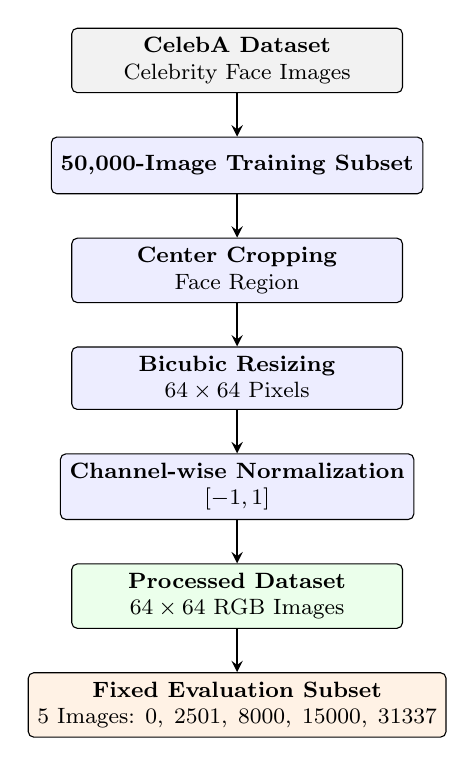
\begin{tikzpicture}[
    node distance=0.55cm,
    box/.style={
        draw,
        rounded corners=2pt,
        align=center,
        minimum width=4.2cm,
        minimum height=0.72cm,
        font=\footnotesize
    },
    source/.style={
        box,
        fill=gray!10
    },
    process/.style={
        box,
        fill=blue!7
    },
    output/.style={
        box,
        fill=green!8
    },
    benchmark/.style={
        box,
        fill=orange!10
    },
    arrow/.style={
        ->,
        >=stealth,
        thick
    }
]

\node[source] (celeba)
    {\textbf{CelebA Dataset}\\Celebrity Face Images};

\node[process, below=of celeba] (subset)
    {\textbf{50,000-Image Training Subset}};

\node[process, below=of subset] (crop)
    {\textbf{Center Cropping}\\Face Region};

\node[process, below=of crop] (resize)
    {\textbf{Bicubic Resizing}\\$64\times64$ Pixels};

\node[process, below=of resize] (normalize)
    {\textbf{Channel-wise Normalization}\\$[-1,1]$};

\node[output, below=of normalize] (dataset)
    {\textbf{Processed Dataset}\\$64\times64$ RGB Images};

\node[benchmark, below=of dataset] (tracked)
    {\textbf{Fixed Evaluation Subset}\\
    5 Images: $0,\;2501,\;8000,\;15000,\;31337$};

\draw[arrow] (celeba) -- (subset);
\draw[arrow] (subset) -- (crop);
\draw[arrow] (crop) -- (resize);
\draw[arrow] (resize) -- (normalize);
\draw[arrow] (normalize) -- (dataset);
\draw[arrow] (dataset) -- (tracked);

\end{tikzpicture}

\caption{Vertical overview of the CelebA dataset preparation pipeline. The 50,000-image subset is center-cropped, resized to $64\times64$, normalized to $[-1,1]$, and evaluated using five fixed benchmark samples for consistent checkpoint-wise comparison.}
\label{fig:dataset-overview}

\end{figure}

% ==============================================================================
% DATASET STATISTICS
% ==============================================================================

% ==============================================================================
% DATASET STATISTICS
% ==============================================================================

\subsection{Dataset Statistics}

The experimental pipeline uses a fixed-resolution subset of the CelebA dataset
to provide a consistent image representation across both Gaussian denoising
and $2\times$ super-resolution tasks. A total of 50{,}000 face images are used
for training. Each image is center-cropped and resized to $64\times64$ pixels
using bicubic interpolation, producing a three-channel RGB representation.
The resulting pixel intensities are normalized independently per channel to
the $[-1,1]$ range, matching the output range of the $\tanh$ activation used
by the WGAN-GP generator.

For reproducible evaluation and consistent checkpoint-wise comparison, five
fixed images are selected using the dataset indices $0$, $2501$, $8000$,
$15000$, and $31337$. These images are retained throughout the experimental
pipeline and are used as fixed benchmark samples for comparing the clean
reference images with their corresponding corrupted or low-resolution inputs
and restored outputs. This fixed evaluation protocol ensures that observed
changes in PSNR and SSIM are attributable to model performance rather than
variation in the evaluation samples.

The principal characteristics of the dataset and its preprocessing
configuration are summarized in Table~\ref{tab:dataset-statistics}.

% ==============================================================================
% TIKZ-BASED DATASET STATISTICS TABLE
% ==============================================================================

\begin{table}[t]
\centering
\caption{Dataset statistics and preprocessing configuration used in the
experimental pipeline.}

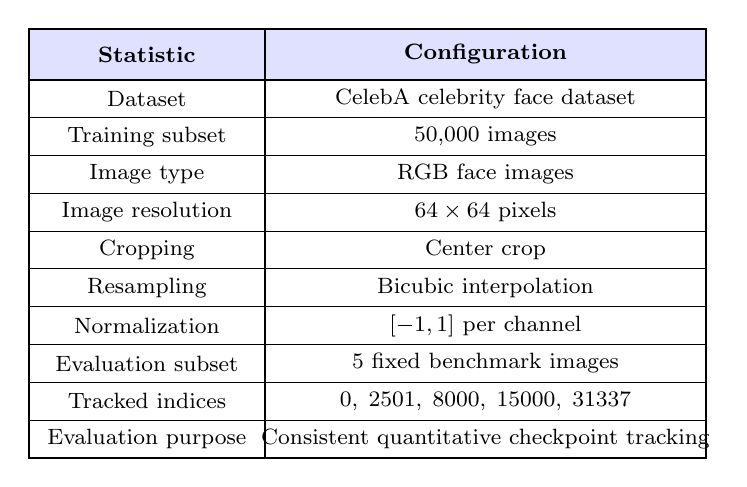
\begin{tikzpicture}

% ------------------------------------------------------------------------------
% Table dimensions
% ------------------------------------------------------------------------------
\def\tablewidth{8.6cm}
\def\leftwidth{3.0cm}
\def\rightwidth{5.6cm}

% ------------------------------------------------------------------------------
% Header
% ------------------------------------------------------------------------------
\fill[blue!12]
    (0,0) rectangle (\tablewidth,-0.65);

\draw[thick]
    (0,0) rectangle (\tablewidth,-0.65);

\draw
    (\leftwidth,0) -- (\leftwidth,-0.65);

\node[
    font=\footnotesize\bfseries,
    align=center
]
at (\leftwidth/2,-0.325)
{Statistic};

\node[
    font=\footnotesize\bfseries,
    align=center
]
at ({\leftwidth+(\rightwidth/2)},-0.325)
{Configuration};

% ------------------------------------------------------------------------------
% Row 1 — Dataset
% ------------------------------------------------------------------------------
\draw
    (0,-0.65) rectangle (\tablewidth,-1.13);

\draw
    (\leftwidth,-0.65) -- (\leftwidth,-1.13);

\node[
    font=\footnotesize,
    align=center
]
at (\leftwidth/2,-0.89)
{Dataset};

\node[
    font=\footnotesize,
    align=center
]
at ({\leftwidth+(\rightwidth/2)},-0.89)
{CelebA celebrity face dataset};

% ------------------------------------------------------------------------------
% Row 2 — Training subset
% ------------------------------------------------------------------------------
\draw
    (0,-1.13) rectangle (\tablewidth,-1.61);

\draw
    (\leftwidth,-1.13) -- (\leftwidth,-1.61);

\node[
    font=\footnotesize,
    align=center
]
at (\leftwidth/2,-1.37)
{Training subset};

\node[
    font=\footnotesize,
    align=center
]
at ({\leftwidth+(\rightwidth/2)},-1.37)
{50,000 images};

% ------------------------------------------------------------------------------
% Row 3 — Image type
% ------------------------------------------------------------------------------
\draw
    (0,-1.61) rectangle (\tablewidth,-2.09);

\draw
    (\leftwidth,-1.61) -- (\leftwidth,-2.09);

\node[
    font=\footnotesize,
    align=center
]
at (\leftwidth/2,-1.85)
{Image type};

\node[
    font=\footnotesize,
    align=center
]
at ({\leftwidth+(\rightwidth/2)},-1.85)
{RGB face images};

% ------------------------------------------------------------------------------
% Row 4 — Image resolution
% ------------------------------------------------------------------------------
\draw
    (0,-2.09) rectangle (\tablewidth,-2.57);

\draw
    (\leftwidth,-2.09) -- (\leftwidth,-2.57);

\node[
    font=\footnotesize,
    align=center
]
at (\leftwidth/2,-2.33)
{Image resolution};

\node[
    font=\footnotesize,
    align=center
]
at ({\leftwidth+(\rightwidth/2)},-2.33)
{$64\times64$ pixels};

% ------------------------------------------------------------------------------
% Row 5 — Cropping
% ------------------------------------------------------------------------------
\draw
    (0,-2.57) rectangle (\tablewidth,-3.05);

\draw
    (\leftwidth,-2.57) -- (\leftwidth,-3.05);

\node[
    font=\footnotesize,
    align=center
]
at (\leftwidth/2,-2.81)
{Cropping};

\node[
    font=\footnotesize,
    align=center
]
at ({\leftwidth+(\rightwidth/2)},-2.81)
{Center crop};

% ------------------------------------------------------------------------------
% Row 6 — Resampling
% ------------------------------------------------------------------------------
\draw
    (0,-3.05) rectangle (\tablewidth,-3.53);

\draw
    (\leftwidth,-3.05) -- (\leftwidth,-3.53);

\node[
    font=\footnotesize,
    align=center
]
at (\leftwidth/2,-3.29)
{Resampling};

\node[
    font=\footnotesize,
    align=center
]
at ({\leftwidth+(\rightwidth/2)},-3.29)
{Bicubic interpolation};

% ------------------------------------------------------------------------------
% Row 7 — Normalization
% ------------------------------------------------------------------------------
\draw
    (0,-3.53) rectangle (\tablewidth,-4.01);

\draw
    (\leftwidth,-3.53) -- (\leftwidth,-4.01);

\node[
    font=\footnotesize,
    align=center
]
at (\leftwidth/2,-3.77)
{Normalization};

\node[
    font=\footnotesize,
    align=center
]
at ({\leftwidth+(\rightwidth/2)},-3.77)
{$[-1,1]$ per channel};

% ------------------------------------------------------------------------------
% Row 8 — Evaluation subset
% ------------------------------------------------------------------------------
\draw
    (0,-4.01) rectangle (\tablewidth,-4.49);

\draw
    (\leftwidth,-4.01) -- (\leftwidth,-4.49);

\node[
    font=\footnotesize,
    align=center
]
at (\leftwidth/2,-4.25)
{Evaluation subset};

\node[
    font=\footnotesize,
    align=center
]
at ({\leftwidth+(\rightwidth/2)},-4.25)
{5 fixed benchmark images};

% ------------------------------------------------------------------------------
% Row 9 — Tracked indices
% ------------------------------------------------------------------------------
\draw
    (0,-4.49) rectangle (\tablewidth,-4.97);

\draw
    (\leftwidth,-4.49) -- (\leftwidth,-4.97);

\node[
    font=\footnotesize,
    align=center
]
at (\leftwidth/2,-4.73)
{Tracked indices};

\node[
    font=\footnotesize,
    align=center
]
at ({\leftwidth+(\rightwidth/2)},-4.73)
{$0,\;2501,\;8000,\;15000,\;31337$};

% ------------------------------------------------------------------------------
% Row 10 — Evaluation purpose
% ------------------------------------------------------------------------------
\draw
    (0,-4.97) rectangle (\tablewidth,-5.45);

\draw
    (\leftwidth,-4.97) -- (\leftwidth,-5.45);

\node[
    font=\footnotesize,
    align=center
]
at (\leftwidth/2,-5.21)
{Evaluation purpose};

\node[
    font=\footnotesize,
    align=center
]
at ({\leftwidth+(\rightwidth/2)},-5.21)
{Consistent quantitative checkpoint tracking};

% ------------------------------------------------------------------------------
% Outer border
% ------------------------------------------------------------------------------
\draw[thick]
    (0,0) rectangle (\tablewidth,-5.45);

\end{tikzpicture}

\label{tab:dataset-statistics}

\end{table}


\section{Methodology}

\subsection{Proposed Methodology}
The proposed framework relies on a sequential multi-stage pipeline designed to extract robust structural priors from a pretrained generative model and use them within conditional diffusion restoration paths, as outlined in Figure~\ref{fig:prop-meth}.
\begin{figure*}[t]
    \centering
    \includegraphics[width=\textwidth]{Fif01_System_Architecture.png}
    \caption{Proposed Methodology}
    \label{fig:prop-meth}
\end{figure*}

\subsubsection{Phase 1 : WGAN-GP Prior Generator}
The generator $G_\theta: \mathbb{R}^{128} \rightarrow \mathbb{R}^{3\times64\times64}$ maps a latent vector $z \sim \mathcal{N}(0, I_{128})$ through five transposed-convolution/BatchNorm/ReLU blocks with a base channel width of 96, doubling spatial resolution at each stage from $4\times4$ to $64\times64$, terminated by a $\tanh$ output. The critic $C_\theta$ mirrors this with strided convolutions, spectral normalization \cite{miyato2018spectral} on every convolutional layer, instance normalization on intermediate layers, and LeakyReLU activations. The critic is optimized via the WGAN-GP objective,
\begin{equation}
\begin{aligned}
\mathcal{L}_C ={}& \mathbb{E}_{\tilde{x}\sim \mathbb{P}_g}[C(\tilde{x})]
- \mathbb{E}_{x\sim \mathbb{P}_r}[C(x)] \\
&+ \lambda_{\text{gp}}\, \mathbb{E}_{\hat{x}}
\big[(\lVert \nabla_{\hat{x}} C(\hat{x})\rVert_2 - 1)^2\big],
\end{aligned}
\label{eq:wgangp}
\end{equation}
with $\lambda_{\text{gp}} = 10$, $\hat{x} = \alpha x + (1-\alpha)\tilde{x}$, and $\alpha \sim \mathcal{U}(0,1)$. The generator is trained using $\mathcal{L}_G = -\mathbb{E}_{z}[C(G(z))]$ every $n_{\text{critic}}=5$ critic updates. An exponential moving average (EMA) copy of $G_\theta$ is maintained throughout training to reduce parameter variance at inference time \cite{yazici2018unusual}.

\subsubsection{Phase 2 : GAN-Guided Conditional U-Net and Diffusion Optimization}
\label{sec:ddim}
Both diffusion U-Nets share a U-Net backbone incorporating FiLM-style timestep conditioning \cite{perez2018film}, bottleneck self-attention, and cross-attention blocks where U-Net spatial features attend to a fixed WGAN-GP feature map ($g$) computed once per sampling chain. Optimization follows a cosine noise schedule ($T=1000$).
\begin{algorithm}[H]
\caption{GAN-Guided Diffusion Training and Sampling}
\label{alg:diffusion_pipeline}
\begin{algorithmic}[1]
\State \textbf{Input:} Frozen generator $G_\theta$, clean data $x_0$, total steps $T=1000$, schedule parameter $s=0.008$.
\State \textbf{Phase 1: Feature Prior Extraction}
\State Sample latent vector $z \sim \mathcal{N}(0, I_{128})$
\State Extract fixed feature map $g \leftarrow G_\theta^{(8\times8)}(z) \in \mathbb{R}^{B \times 384 \times 8 \times 8}$
\State \textbf{Phase 2: Training Objective}
\State Sample timestep $t \sim \mathcal{U}\{0, \dots, T-1\}$ and noise $\varepsilon \sim \mathcal{N}(0, I)$
\State Compute forward diffusion: $x_t = \sqrt{\bar\alpha_t}x_0 + \sqrt{1-\bar\alpha_t}\,\varepsilon$
\State Compute cross-attention: $Q(x_t)$, $K(g)$, $V(g)$
\State \quad $\text{TextCrossAttn}(x_t, g) = x_t + W_o \Big[\text{softmax}\Big(\frac{Q(x_t) K(g)^\top}{\sqrt{d}}\Big) V(g)\Big]$
\State Minimize objective: $\mathcal{L}_{\text{diff}} = \mathbb{E}\big[\lVert \varepsilon - \epsilon_\phi(x_t, t, g) \rVert_2^2\big]$
\State \textbf{Phase 3: DDIM Inference (Single-Pass Prior Reuse)}
\State Initialize $x_{t_{\text{start}}}$ (via corrupted input injection for denoising or noise for SR)
\For{$t = t_{\text{start}}, \dots, 1$}
\State Predict clean image: $\hat{x}_0 = \frac{x_t - \sqrt{1-\bar\alpha_t}\,\epsilon_\phi(x_t, t, g)}{\sqrt{\bar\alpha_t}}$ (clipped to $[-1, 1]$)
\State Update deterministically to $x_{t'}$ using fixed $g$
\EndFor
\end{algorithmic}
\end{algorithm}

\subsection{Experimental Setup}
The implementation is evaluated across stable configurations and optimized hyperparameters to resolve prior pipeline instabilities:
% \begin{enumerate}
%     \item \textbf{Learning-Rate Rebalancing:} $\text{LR}_G$ and $\text{LR}_D$ are set symmetrically to $2\times10^{-4}$ (Adam, $\beta_1{=}0.0, \beta_2{=}0.9$) to prevent critic dominance and gradient divergence.
%     \item \textbf{Corrected DDIM Initialization:} For denoising, the reverse chain initializes by forward-diffusing the corrupted observation to $t_{\text{start}}=150$ rather than starting from unconditioned noise.
%     \item \textbf{Calibrated Corruption:} Gaussian noise severity is set to $\sigma=0.15$ on the $[-1,1]$ scale, matching the $t_{\text{start}}=150$ timestep under the cosine schedule.
%     \item \textbf{EMA Smoothing:} The EMA decay rate is raised to $0.9999$ to suppress high-frequency parameter noise.
% \end{enumerate}

\begin{table}[t]
\centering
\caption{Training hyperparameters for the restoration pipeline.}
\label{tab:hparams}
\begin{tabular}{@{}ll@{}}
\toprule
\textbf{Parameter} & \textbf{Value} \\
\midrule
Image resolution & $64\times64$ \\
Training subset size & 50{,}000 images \\
Batch size (WGAN-GP / Diffusion) & 64 / 32 \\
\midrule
\multicolumn{2}{@{}l}{\textit{WGAN-GP Prior}} \\
Latent dimension $z$ & 128 \\
Generator / critic width & 96 \\
Optimizer ($G$ and $D$) & Adam ($\beta_1{=}0.0,\beta_2{=}0.9$) \\
Learning rate ($\text{LR}_G$, $\text{LR}_D$) & $2\times10^{-4}$, $2\times10^{-4}$ \\
Gradient penalty $\lambda_{\text{gp}}$ & 10 \\
\midrule
\multicolumn{2}{@{}l}{\textit{Diffusion Backbone}} \\
Timesteps $T$ (Cosine schedule) & 1000 \\
DDIM sampling steps & 50 \\
Optimizer & AdamW (wd $=10^{-4}$) \\
EMA decay & 0.9999 \\
\midrule
\multicolumn{2}{@{}l}{\textit{Task Specifications}} \\
Denoising epochs / $\sigma$ / $t_{\text{start}}$ & 30 / 0.15 / 150 \\
Super-resolution epochs / factor & 25 / $2\times$ \\
\bottomrule
\end{tabular}
\end{table}

% \begin{figure*}[t]
% \centering
% \experimentfigure[width=\textwidth]{Fig05_Model_Scale_Configuration.png}
% \caption{Model scale and experimental configuration. The diffusion U-Nets dominate parameter volume, while the WGAN-GP components manage prior learning.}
% \label{fig:model-scale}
% \end{figure*}

\subsection{System Architecture}
The framework features a hybrid design where a pre-trained generator acts as a reusable prior. The complete system architecture is shown in Figure~\ref{fig:prop-meth}.


\subsection{Evaluation Metrics}
Restoration performance is measured using Peak Signal-to-Noise Ratio (PSNR) and Structural Similarity Index (SSIM) \cite{wang2004ssim}. These metrics are computed on the five tracked faces between the ground-truth clean image and both the degraded inputs and the final diffusion-restored outputs to quantify the improvement achieved by the GAN-guided refinement process.

\section{Results}

\subsection{Training Dynamics}

\begin{figure*}[t]
\centering
\experimentfigure[width=\textwidth]{Fig02_Training_Loss_Curves.png}
\caption{Training loss curves for the v3 pipeline. Left: WGAN-GP generator (solid) and critic (dashed) losses over 100 epochs (first 50 shown), converging smoothly under equal $2\times10^{-4}$ learning rates. Center: denoising U-Net $\epsilon$-prediction MSE loss over 30 epochs. Right: super-resolution U-Net $\epsilon$-prediction MSE loss over 25 epochs.}
\label{fig:losses}
\end{figure*}

Figure~\ref{fig:losses} shows the WGAN-GP generator/critic loss curves and the diffusion U-Net MSE loss curves over training. The WGAN-GP critic loss increases smoothly from $-23.99$ at epoch 1 toward $-4.71$ by epoch 50, while the generator loss decreases monotonically from $36.65$ to $18.44$ over the same period, indicating stable, non-oscillatory adversarial convergence under the corrected symmetric learning rates -- in contrast to the divergence behavior diagnosed in the v2 configuration. Both diffusion U-Nets show smooth, monotonically-decreasing MSE noise-prediction loss: the denoising U-Net converges from $0.079$ to $0.037$ over 30 epochs, and the super-resolution U-Net converges from $0.060$ to $0.014$ over 25 epochs, the latter converging to a substantially lower absolute loss, consistent with super-resolution being a better-conditioned inverse problem (bicubic upsampling already recovers most low-frequency content) than blind Gaussian denoising at the evaluated noise level.

Per-epoch validity checks (finiteness, per-sample pixel standard deviation $>10^{-3}$, dynamic range $>10^{-2}$) confirm that the generator does not collapse at any of the ten logged WGAN-GP checkpoints (epochs 10, 20, \ldots, 50); sample standard deviation increases steadily from $0.430$ at epoch 10 to $0.476$ at epoch 50, indicating increasing output diversity/contrast as training progresses.

\subsection{Restoration Quality}
Table~\ref{tab:results} reports PSNR and SSIM, averaged over the five tracked faces, before and after diffusion-based restoration for both tasks.

\begin{table}[t]
\centering
\caption{Restoration results on 5 tracked CelebA faces (mean values; see Table~\ref{tab:persample} for per-sample values).}
\label{tab:results}
\footnotesize
\begin{tabular}{@{}p{2.05cm}p{1.55cm}cc@{}}
\toprule
\textbf{Task} & \textbf{Stage} & \textbf{PSNR (dB)} & \textbf{SSIM} \\
\midrule
\multirow{2}{2.05cm}{Denoising \\ ($\sigma{=}0.15$)} & Corrupted input & 22.76 & 0.6755 \\
 & Restored & \textbf{27.17} & \textbf{0.8429} \\
\addlinespace
\multicolumn{2}{@{}l}{\quad $\Delta$ (input $\rightarrow$ restored)} & \multicolumn{2}{c}{+4.40 dB\ /\ +0.167} \\
\midrule
\multirow{2}{2.05cm}{Super-res. \\ ($2\times$)} & Bicubic baseline & 27.24 & 0.9122 \\
 & Restored & \textbf{30.94} & \textbf{0.9566} \\
\addlinespace
\multicolumn{2}{@{}l}{\quad $\Delta$ (baseline $\rightarrow$ restored)} & \multicolumn{2}{c}{+3.70 dB\ /\ +0.044} \\
\bottomrule
\end{tabular}
\end{table}

\begin{table}[t]
\centering
\caption{Per-sample PSNR (dB) on the 5 fixed tracked faces.}
\label{tab:persample}
\begin{tabular}{@{}lcccc@{}}
\toprule
\textbf{Sample} & \textbf{Noisy} & \textbf{Denoised} & \textbf{Bicubic} & \textbf{SR out} \\
\midrule
S1 & 23.0 & 26.2 & 24.8 & 27.5 \\
S2 & 22.8 & 26.8 & 28.8 & 31.2 \\
S3 & 22.6 & 27.6 & 27.9 & 33.4 \\
S4 & 22.6 & 27.2 & 29.0 & 30.6 \\
S5 & 22.7 & 28.0 & 25.7 & 32.0 \\
\midrule
Mean & 22.76 & 27.17 & 27.24 & 30.94 \\
\bottomrule
\end{tabular}
\end{table}

\begin{figure*}[t]
\centering
\experimentfigure[width=\textwidth]{Fig03_Metric_Heatmap.png}
\caption{Per-sample and mean PSNR (left) and SSIM (right) before and after restoration. Lighter cells indicate higher metric values; both tasks improve consistently across the five fixed tracked samples.}
\label{fig:metric-heatmap}
\end{figure*}

\begin{figure*}[t]
\centering
\experimentfigure[width=\textwidth]{Fig04_Restoration_Gain.png}
\caption{Per-sample restoration gains in PSNR and SSIM for denoising and super-resolution. Every tracked sample improves under both restoration tasks.}
\label{fig:restoration-gain}
\end{figure*}

Figures~\ref{fig:metric-heatmap} and~\ref{fig:restoration-gain} visualize the absolute metric values and their per-sample gains, respectively. Every one of the five tracked faces shows a positive PSNR gain under both tasks, with no degenerate or negative-improvement samples, which we take as evidence that the corrected pipeline generalizes the restoration behavior across faces with varying pose, lighting, and occlusion (e.g., the sunglasses-occluded sample in the tracked set) rather than overfitting to a subset of easy cases. The super-resolution task achieves a substantially higher absolute PSNR/SSIM than denoising, both before and after restoration, consistent with $2\times$ bicubic downsampling being a milder, more information-preserving degradation than additive Gaussian noise at $\sigma=0.15$.

\subsection{Qualitative Observations}

\begin{figure*}[t]
\centering
\experimentfigure[width=\textwidth]{Fig06_Denoising.png}
\caption{Denoising results on the 5 fixed tracked faces. Top: clean reference. Middle: corrupted input ($\sigma=0.15$ Gaussian noise). Bottom: GAN-guided diffusion restoration via the corrected DDIM initialization (Section~\ref{sec:ddim}).}
\label{fig:denoise_tracked}
\end{figure*}

\begin{figure*}[t]
\centering
\experimentfigure[width=\textwidth]{Fig07_Super_Resolution.png}
\caption{Super-resolution results on the 5 fixed tracked faces. Top: clean reference. Middle: $2\times$ bicubic downsample/upsample baseline. Bottom: GAN-guided diffusion $2\times$ super-resolution output.}
\label{fig:sr_tracked}
\end{figure*}

Figures~\ref{fig:denoise_tracked} and~\ref{fig:sr_tracked} show the tracked-face grids (five faces $\times$ three rows: clean / degraded / restored). Visual inspection shows that the GAN-guided diffusion denoiser removes the majority of visible speckle noise while preserving identity-relevant structure (eyes, hair boundary, mouth), and the super-resolution model recovers plausible high-frequency texture (hair strands, skin texture) not present in the blurry bicubic input, without introducing the checkerboard artifacts commonly associated with naive transposed-convolution upsamplers.

\section{Discussion}

\subsection{Why a Frozen, Once-Per-Chain GAN Prior Stabilizes Sampling}
The central architectural lesson from the v2-to-v3 transition is that the GAN conditioning signal $g$ must be treated as a \emph{fixed} context for the full DDIM trajectory rather than resampled at each of the 50 reverse steps. Since DDIM sampling is a deterministic map from $x_T$ (or $x_{t_{\text{start}}}$) to $x_0$ conditioned on a sequence of network evaluations, allowing $g$ to vary stochastically between steps effectively turns the deterministic trajectory into a piecewise-inconsistent one, where the model receives conflicting semantic guidance at successive timesteps; the corrected implementation removes this inconsistency by computing $g$ once, immediately before the reverse loop begins, and reusing it for every DDIM update.

\subsection{Learning-Rate Symmetry in WGAN-GP}
The 4x generator/critic LR imbalance diagnosed in v2 is a plausible source of instability given the WGAN-GP loss landscape: an overly fast critic relative to the generator can drive the critic into a regime where its gradients with respect to generator-produced samples become uninformative or saturate, since the critic ``overfits'' to distinguishing the current generator's slightly-imperfect samples faster than the generator can adapt. Restoring the standard symmetric $2\times10^{-4}/2\times10^{-4}$ configuration recommended in the original WGAN-GP paper \cite{gulrajani2017wgangp} resolves this without any architectural change, stressing that hyperparameter symmetry, not model capacity, was the binding constraint in the earlier iteration.

\subsection{Limitations}
This study is limited in several respects. First, evaluation is restricted to five fixed tracked faces; while this enables precise before/after tracking, it does not provide a population-level estimate of restoration quality or its variance, and a full evaluation would benefit from a held-out test set of several hundred to several thousand faces with confidence intervals. Second, no perceptual metric (e.g., LPIPS \cite{zhang2018lpips}, present in the v1 evaluation harness but not carried through to v3) or FID score \cite{heusel2017fid} is reported for the final pipeline, both of which are known to correlate better with human perceptual judgments of face realism than PSNR/SSIM alone. Third, the corruption model for denoising is restricted to a single, fixed Gaussian noise level ($\sigma=0.15$); robustness across a range of corruption severities is untested. Fourth, no ablation isolates the marginal contribution of the GAN cross-attention conditioning itself (i.e., an unconditioned diffusion baseline with the cross-attention block removed) from the other v2$\rightarrow$v3 fixes, so the reported gains should be attributed to the corrected pipeline as a whole rather than to GAN guidance in isolation.

\section{Conclusion}

We presented a GAN-guided conditional diffusion pipeline for face image denoising and super-resolution, in which a frozen WGAN-GP generator's intermediate feature map conditions a diffusion U-Net via cross-attention, computed once per sampling chain and held fixed across all DDIM reverse steps. Through an iterative, diagnosis-driven development process across three implementation stages, we identified and corrected four specific instabilities -- generator/critic learning-rate imbalance, incorrect DDIM initialization for denoising, an uncalibrated corruption level, and an insufficiently smooth EMA schedule -- that separated an unstable v2 configuration from a stable, consistently-improving v3 configuration. On five tracked CelebA faces, the corrected pipeline improves Gaussian-denoising PSNR by 4.40 dB (SSIM +0.167) and super-resolution PSNR by 3.70 dB (SSIM +0.044) over their respective naive baselines, with every tracked sample showing positive improvement on both metrics. Future work should extend evaluation to a larger held-out test set with perceptual (LPIPS/FID) metrics, ablate the GAN cross-attention conditioning against an unconditioned diffusion baseline under matched compute, and evaluate robustness across a range of corruption severities and real (non-synthetic) degradations.

\begin{thebibliography}{00}

\bibitem{goodfellow2014gan} I. Goodfellow, J. Pouget-Abadie, M. Mirza, B. Xu, D. Warde-Farley, S. Ozair, A. Courville, and Y. Bengio, ``Generative adversarial nets,'' in \textit{Advances in Neural Information Processing Systems (NeurIPS)}, 2014.

\bibitem{gulrajani2017wgangp} I. Gulrajani, F. Ahmed, M. Arjovsky, V. Dumoulin, and A. C. Courville, ``Improved training of Wasserstein GANs,'' in \textit{Advances in Neural Information Processing Systems (NeurIPS)}, 2017.

\bibitem{ho2020ddpm} J. Ho, A. Jain, and P. Abbeel, ``Denoising diffusion probabilistic models,'' in \textit{Advances in Neural Information Processing Systems (NeurIPS)}, 2020.

\bibitem{sohl2015deep} J. Sohl-Dickstein, E. Weiss, N. Maheswaranathan, and S. Ganguli, ``Deep unsupervised learning using nonequilibrium thermodynamics,'' in \textit{Proc. Int. Conf. Machine Learning (ICML)}, 2015.

\bibitem{dhariwal2021diffusion} P. Dhariwal and A. Nichol, ``Diffusion models beat GANs on image synthesis,'' in \textit{Advances in Neural Information Processing Systems (NeurIPS)}, 2021.

\bibitem{radford2015dcgan} A. Radford, L. Metz, and S. Chintala, ``Unsupervised representation learning with deep convolutional generative adversarial networks,'' \textit{arXiv preprint arXiv:1511.06434}, 2015.

\bibitem{karras2019stylegan} T. Karras, S. Laine, and T. Aila, ``A style-based generator architecture for generative adversarial networks,'' in \textit{Proc. IEEE/CVF Conf. Computer Vision and Pattern Recognition (CVPR)}, 2019.

\bibitem{song2020ddim} J. Song, C. Meng, and S. Ermon, ``Denoising diffusion implicit models,'' in \textit{Proc. Int. Conf. Learning Representations (ICLR)}, 2021.

\bibitem{nichol2021improved} A. Nichol and P. Dhariwal, ``Improved denoising diffusion probabilistic models,'' in \textit{Proc. Int. Conf. Machine Learning (ICML)}, 2021.

\bibitem{saharia2022sr3} C. Saharia, J. Ho, W. Chan, T. Salimans, D. J. Fleet, and M. Norouzi, ``Image super-resolution via iterative refinement,'' \textit{IEEE Trans. Pattern Analysis and Machine Intelligence}, 2022.

\bibitem{saharia2022palette} C. Saharia, W. Chan, H. Chang, C. Lee, J. Ho, T. Salimans, D. Fleet, and M. Norouzi, ``Palette: Image-to-image diffusion models,'' in \textit{Proc. ACM SIGGRAPH}, 2022.

\bibitem{meng2021sdedit} C. Meng, Y. He, Y. Song, J. Song, J. Wu, J.-Y. Zhu, and S. Ermon, ``SDEdit: Guided image synthesis and editing with stochastic differential equations,'' in \textit{Proc. Int. Conf. Learning Representations (ICLR)}, 2022.

\bibitem{xiao2021ddgan} Z. Xiao, K. Kreis, and A. Vahdat, ``Tackling the generative learning trilemma with denoising diffusion GANs,'' in \textit{Proc. Int. Conf. Learning Representations (ICLR)}, 2022.

\bibitem{miyato2018spectral} T. Miyato, T. Kataoka, M. Koyama, and Y. Yoshida, ``Spectral normalization for generative adversarial networks,'' in \textit{Proc. Int. Conf. Learning Representations (ICLR)}, 2018.

\bibitem{yazici2018unusual} Y. Yaz{\i}c{\i}, C.-S. Foo, S. Winkler, K.-H. Yap, G. Piliouras, and V. Chandrasekhar, ``The unusual effectiveness of averaging in GAN training,'' in \textit{Proc. Int. Conf. Learning Representations (ICLR)}, 2019.

\bibitem{perez2018film} E. Perez, F. Strub, H. de Vries, V. Dumoulin, and A. Courville, ``FiLM: Visual reasoning with a general conditioning layer,'' in \textit{Proc. AAAI Conf. Artificial Intelligence}, 2018.

\bibitem{wang2004ssim} Z. Wang, A. C. Bovik, H. R. Sheikh, and E. P. Simoncelli, ``Image quality assessment: From error visibility to structural similarity,'' \textit{IEEE Trans. Image Processing}, vol. 13, no. 4, pp. 600--612, 2004.

\bibitem{zhang2018lpips} R. Zhang, P. Isola, A. A. Efros, E. Shechtman, and O. Wang, ``The unreasonable effectiveness of deep features as a perceptual metric,'' in \textit{Proc. IEEE/CVF Conf. Computer Vision and Pattern Recognition (CVPR)}, 2018.

\bibitem{heusel2017fid} M. Heusel, H. Ramsauer, T. Unterthiner, B. Nessler, and S. Hochreiter, ``GANs trained by a two time-scale update rule converge to a local Nash equilibrium,'' in \textit{Advances in Neural Information Processing Systems (NeurIPS)}, 2017.

\end{thebibliography}

\end{document}
